{\fontsize{12}{14}\selectfont 

La parte I dell'esperienza consiste nel misurare la forza di Lorentz al variare della corrente. 
\\
Si è prima pesato il magnete A sulla bilancia, ottenendo una misura di $M_0 = (158.30 \pm 0.01)g$, poi è stata montata la Current Balance Main Unit con il circuito SF42 in quanto è il più lungo dei circuiti stampati, nonchè quello con il minore errore relativo sulla lunghezza e non varierà durante questa parte dell'esperimento.
Il circuito è stato inserito nel magnete in modo tale da formare un angolo di 90°, avendo cura di non metterli a contatto.
\\
Dopo aver acceso il generatore in modalità corrente ed averlo impostato a 0A è stato montato il circuito nel modo seguente:

\par
\begin{center}
    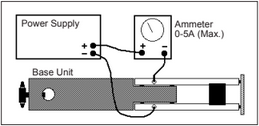
\includegraphics[width=8cm]{Figures/Circuito.png}
\end{center}
\par

Quindi è stato misurato il peso del magnete al variare della corrente a passi di $0.5$A fino ad arrivare a $4.5$A per non superare la portata di 5A dell'amperometro. 
\\
Per verificare la ripetibilità delle misure, il circuito è stato completamente smontato e ricostruito prima di prendere un secondo set.
\\
Ogni misura è stata sottratta al peso $M_0$ per ricavare la variazione di peso dovuta alla forza di Lorentz ed è poi stata plottata in funzione della corrente.
\par}